\section{Server}
\label{server}
Wie in Abschnitt \ref{app_architecture} beschrieben, müssen die aufgezeichneten Daten der Clientbibliothek weiter verarbeitet werden. % TODO nochmal etwas genauer

Im Folgenden werden die serverseitigen Komponenten, virtuelle Maschine, Datenbank und HTTP-Server, vorgestellt. 



\subsection{Virtuelle Maschine}

\subsubsection{Konfiguration \label{sec:vm-config}}

Als Betriebssystem für den Server dient ein Debian in der Version 7.0. Der Maschine wurde 1 Prozessorkern und 512 MB RAM zugewiesen. Änderungen können im Vagrantfile, siehe Abschnitt \ref{vagrant}, oder der Virtual Box-Konfiguration vorgenommen werden. 

Folgende Software wurde für den Entwicklungsprozess verwendet. 
\begin{description}
	\item[OpenSSH-Server\footnotemark]\footnotetext{http://www.openssh.org/} 
Das Programmpaket für die \emph{Secure Shell} beinhaltet alle Softwaretools um Dateien zwischen Host- und Gast- System auszutauschen (scp, sftp) oder sich darauf zu verbinden (ssh). Das Softwarepaket ist notwendig um beispielsweise Vagrant (siehe Abschnitt \ref{sec:Vagrant}) betreiben zu können. 

	\item[MySQL Server\footnotemark]\footnotetext{http://www.mysql.de/products/community/}
Zur persistenten Speicherung der Nutzdaten wird MySQL verwendet. MySQL bietet sich an, da es Verbreitung und Sicherheit bietet, sowie von Oracle als kommerzielles, wie auch Open Source-Derivat entwickelt wird. Das Projekt nutzt die Community-Server-Edition.
	
	\item[Node.js\footnotemark und NPM\footnotemark]\footnotetext{http://nodejs.org/}\footnotetext{https://www.npmjs.org/}
Node.js, kurz Node, ist eine Platform basierend auf der JavaScript Laufzeitumgebung des Browsers Chrome. Die Intension von Node ist es schnelle, skalierbare Netzwerkanwendung entwickeln zu können. Dabei wird ein ereignisgetriebenes, nicht blockierendes Eingabe-/Ausgabesystem verwendet. Der Node Package Manager, kurz NPM, wird verwendet um weitere Abhängigkeiten der Anwendung zu verwalten.
	
\end{description}

\subsubsection{Vagrant \label{sec:Vagrant}}
\label{vagrant}
Um die Bereitstellung der Serverumgebung zu vereinfachen wurde die virtuelle Maschine mittels Vagrant\footnote{Vagrant: http://www.vagrantup.com/} konfiguriert. Vagrant ist ein Kommandozeilenwerkzeug um schnell reproduzierbare Entwicklungsumgebungen zu schaffen und diese später zu verteilen oder zu exportieren. Dabei wird Virtual Box\footnote{https://www.virtualbox.org/} als Virtualisierungssoftware eingesetzt. Aber auch VMware wird unterstützt. 

Die eigene VM wird mittels einer VM-Schablone (die eigentliche VM) und einer Konfigurationsdatei geladen, die alle Eigenschaften der VM bereithält, wie zum Beispiel Portweiterleitungen. Die Schablone kann demnach bereits einige Standardsoftwarepakete beinhalten. 

Auf dem Host-System können die gewohnten Entwicklungswerkzeuge eingesetzt werden, da der Ordner, indem Vagrant konfiguriert wurd, mit dem Ordner /Vagrant auf dem Gast-System synchronisiert wird. 

Auch die Entwicklung von Software mittels einer Vagrant VM ergibt einen gut zu bedienenden Arbeitsfluss. So ist es beispielsweise möglich mittels \textbf{vagrant up} und \textbf{vagrant ssh} die Maschine zu starten und darauf zu verbinden, ohne dabei extra overhead, wie zum Beispiel Fenster, zu erzeugen. Die SSH-Credentials folgen dem \textit{Convention over Configuration}-Paradigma. Username, sowie Passwort lauten standardmäßig vagrant. 

\subsection{Datenbank}

\subsubsection{Datenbank-Modell}
Das Datenbankmodell wurde mit Hilfe des MySQL Workbench erstellt. Die Abbildung \ref{figure-db-model} zeigt das Ergebnis.
\begin{figure}[h!]
	\centering
	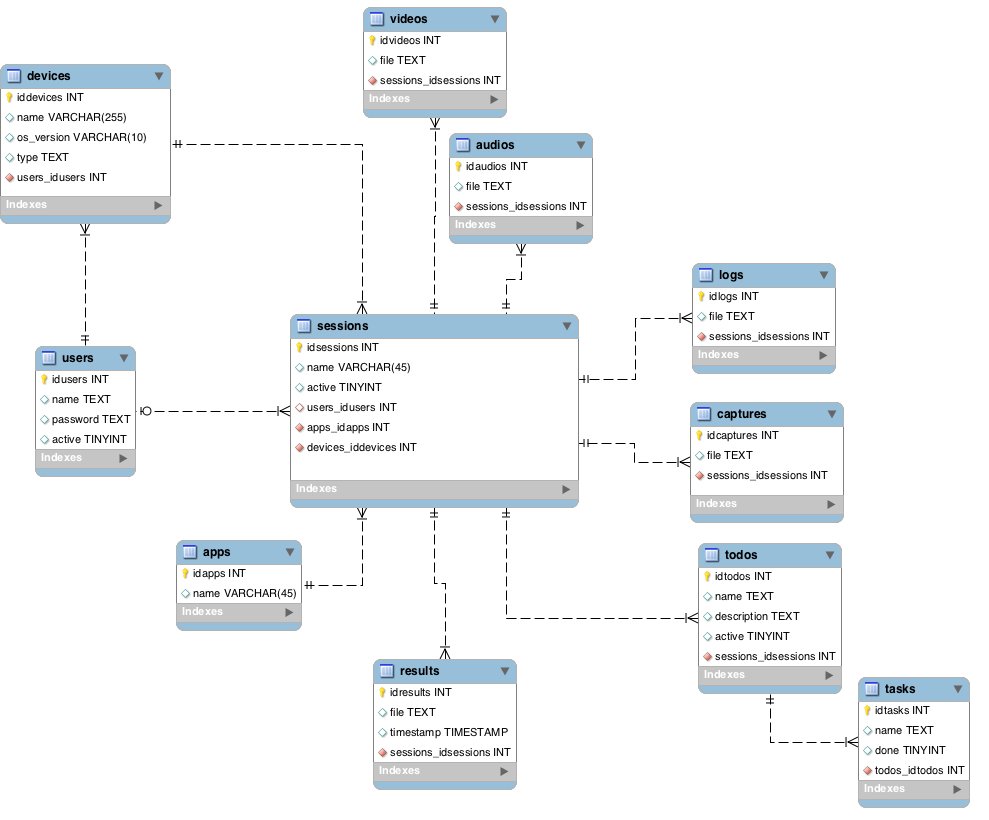
\includegraphics[width=\linewidth,keepaspectratio]{img/db_model.png}
	\caption{Datenbank Modell}
	\label{figure-db-model}
\end{figure}


\subsection{HTTP-Server und Middleware}
Die serverseitige Logik wurde mit dem Express-Framework\footnote{http://expressjs.com/} umgesetzt. Folglich wurde serverseitig Javascript eingsetzt. Javascript eigenet sich sehr gut für Programmierschnittstellen und HTTP-Anfragen. Nicht nur, da Javascript aus dem Web nicht mehr wegzudenken ist, sondern auch da es komplett asynchron programmiert werden kann. 

Das Express-Framework stellt die grundlegenden Funktionen eines Web-, bzw. HTTP-Servers bereit. Ein minimaler HTTP-Server ist im Listing \ref{minimal_node_http_server} zu sehen. Eine Express-Anwendung stellt Pfade, sog. \emph{routes}, zur Verfügung auf die der HTTP-Server reagiert. Im Listing wird Zeile 23 wird eine solcher Pfad angelegt. 

\begin{lstlisting}[label=minimal_node_http_server,language=Java, caption=Minimaler Node-HTTP-Server]
/**
 * Module dependencies.
 */
var express = require('express');
var routes = require('./routes');
var http = require('http');
var path = require('path');
var app = express();

// environments config
app.set('port', process.env.PORT || 3000);
app.set('views', path.join(__dirname, 'views'));
app.set('view engine', 'ejs');
app.use(express.favicon());
app.use(express.logger('dev'));
app.use(express.json());
app.use(express.urlencoded());
app.use(express.methodOverride());
app.use(app.router);
app.use(express.static(path.join(__dirname, 'public')));

// simple test route
app.get('/ping', routes.pong);


// server take off
http.createServer(app).listen(app.get('port'), function(){
  console.log('Express server listening on port ' + app.get('port'));
});
\end{lstlisting}

Im Projektordner befindet sich der Unterordner \textbf{serverside}. In diesem finden sich alle Serverdateien. Die Baumstruktur aus Abbildung \ref{fig:server-tree} zeigt die Ordnerhierachie des Projekts.

Im Ordner \textit{node\_modules} befinden sich alle weiteren Module die für die Serveranwendung benötigt und durch NPM verwaltet werden (Details zu den Modulen finden sich im Abschnitt \ref{sec:node-mudules}). 

Im Unterordner \textit{controllers} werden die Web- und API-Routen-Handler gehalten. Diese werden in \textbf{app.js} als Callback-Funktionen aufgerufen (der Abschnitt \ref{sec: api} beschreibt die Routen detailliert). Im Ordner \textit{public} werden alle Dateien für die Browseranwendung (clientseitiges Javascript, CSS, Bilder und Schriftarten) angelegt und gehalten. Letztlich werden die HTML-Views im Unterordner \textit{views} gehalten. 

Die Ordnerstruktur entspricht weitestgehend der Standardkonfiguration einer Express-Web-Anwendung.

\begin{figure}[h!]
	\centering
			\begin{minipage}[c]{\textwidth} %Ordnerstruktur in Minipage damit die zusammengehalten wird
				\dirtree{%
				 .1 /serverside.
				 .2 classes.
				 .2 controllers.
				 	.3 api.
				 .2 node\_modules.
				 .2 public.
				 	.3 css.
				 	.3 fonts.
				 	.3 img.
				 	.3 js.
				 .2 uploads.
				 .2 views.
				}
			\end{minipage}
	\caption{Ordnerstruktur des Servers}
	\label{fig:server-tree}
\end{figure}

Der Node-Server kann mittels des Befehls \textbf{node app.js}, bzw. \textbf{npm start}, ausgeführt werden und lauscht, wenn nicht anders angegeben, auf den Port 3000. 

\subsubsection{Node Module \label{sec:node-mudules}}

Wie im Abschnitt \ref{sec:vm-config} beschrieben werden alle Abhängigkeit für den Node-Server mittels NPM verwaltet. NPM funktioniert wie andere Paketmanager. Auf Im Normalfall wird NPM mit Node ausgeliefert und installiert. 

Im Ordner \textit{serverside} befindet sich die Datei \emph{package.json}. Diese Datei enthält alle benötigten Abhängigkeiten im JSON\footnote{http://www.json.org/}-Format. Das Listing \ref{node-packages} zeigt das Paket-JSON-Objekt. Neben den Projektinformationen beinhaltet es ein weiteres Objekt, \emph{dependencies}. 

In diesem sind die jeweiligen Abhängigkeiten zu den verwendeten Modulen, zum Beispiel das Express-Framework, enthalten. Jeder Eintrag besteht aus dem Namen des Moduls und der gewünschten Version. Das \emph{*} bedeutet das die aktuellste Version genutzt werden soll. Mittels des Befehls \textbf{npm install} im Ordner \textit{serverside} können die Abhängigkeiten installiert werden. 

\begin{lstlisting}[label=node-packages,language=Java, caption=Abhängigkeiten der Node-Anwendung]
{
    "name": "hipsterbility-server",
    "version": "0.0.1",
    "private": true,
    "scripts": {
    "start": "node app.js"
    },
    "dependencies": {
    "express": "*",
	"jade": "*",
	"mysql" : "*",
    "avconv":"*",
    "passport":"*",
    "passport-local":"*",
    "string":"*",
    "mkdirp":"*"

  }
}
\end{lstlisting}

\subsubsection{Webbasiertes Verwaltungstool}

Nach Abschnitt \ref{sec: zielsetzung} ist es Ziel eine zentrale Komponente zur Verfügung zu stellen mit der Tests verwaltet werden können. Zudem wurde ein rudimentäres Login-System implementiert. An dieser Stelle sei gesagt, dass die webbasierte Verwaltung nur skizziert ist. Eine vollständige, auf Sicherheit geprüfte und nach allen heutigen Webstandards aufbauende, Webanwendung steht nicht zur Verfügung. Dies ist im Rahmen dieser Semesterarbeit nicht entstanden und auch nicht das Anliegen dieser Arbeit. Vielmehr ist es ein Proof-Of-Concept. 

\begin{figure}[h!]
	\centering
		
\includegraphics[width=\linewidth,keepaspectratio]{img/index-page.png}
	\caption{Index-Seite der Anwendung}
	\label{fig: index-page}
\end{figure}

\begin{figure}[h!]
	\centering
		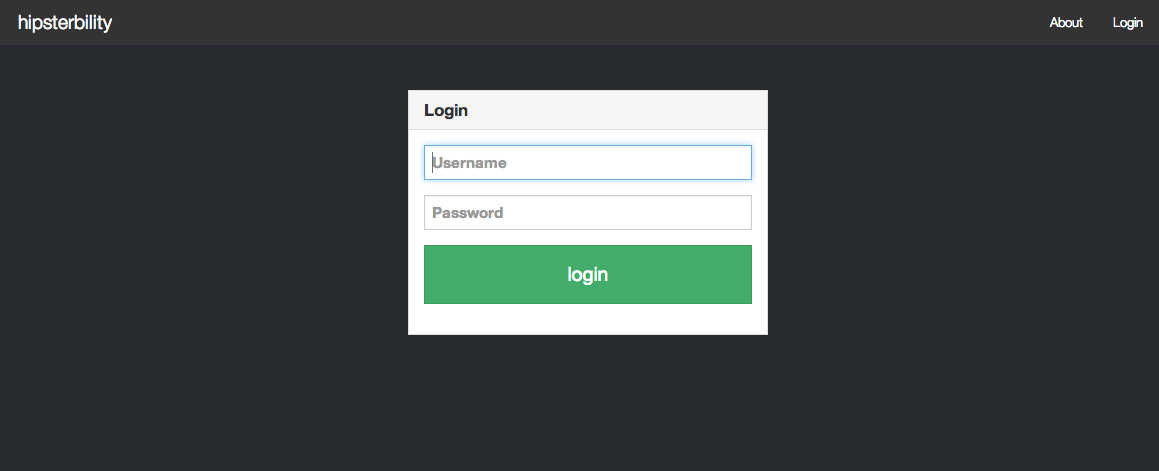
\includegraphics[width=\linewidth,keepaspectratio]{img/login-page.png}
	\caption{Login-Seite der Anwendung}
	\label{fig: login-page}
\end{figure}

\begin{figure}[h!]
	\centering
		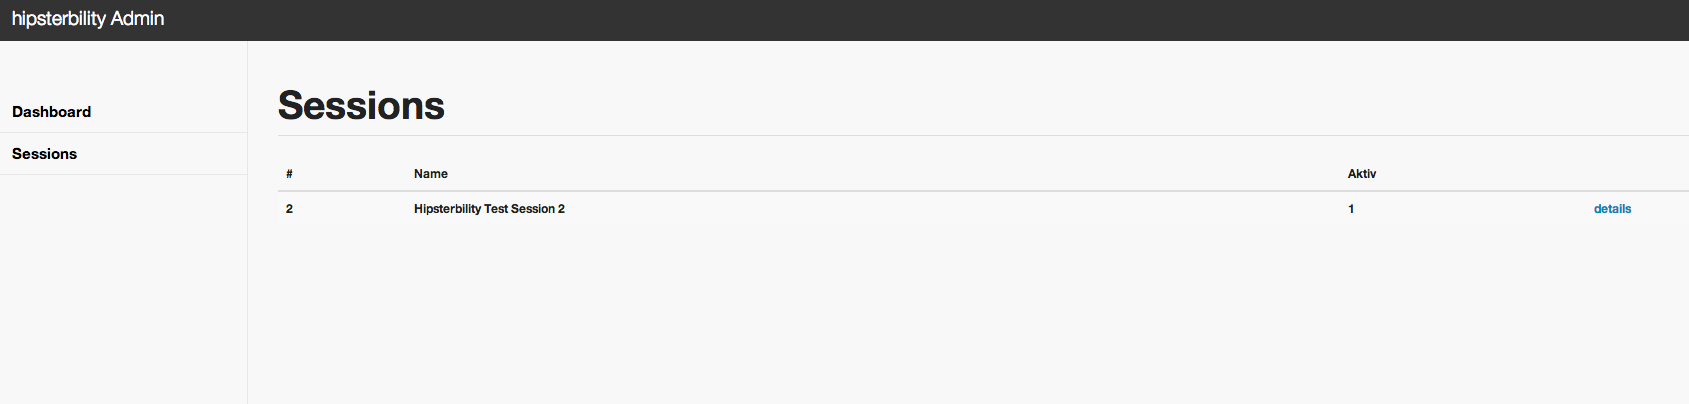
\includegraphics[width=\linewidth,keepaspectratio]{img/sessions-page.png}
	\caption{Listenansicht für Testsessions}
	\label{fig: sessions-page}
\end{figure}

\begin{figure}[h!]
	\centering
		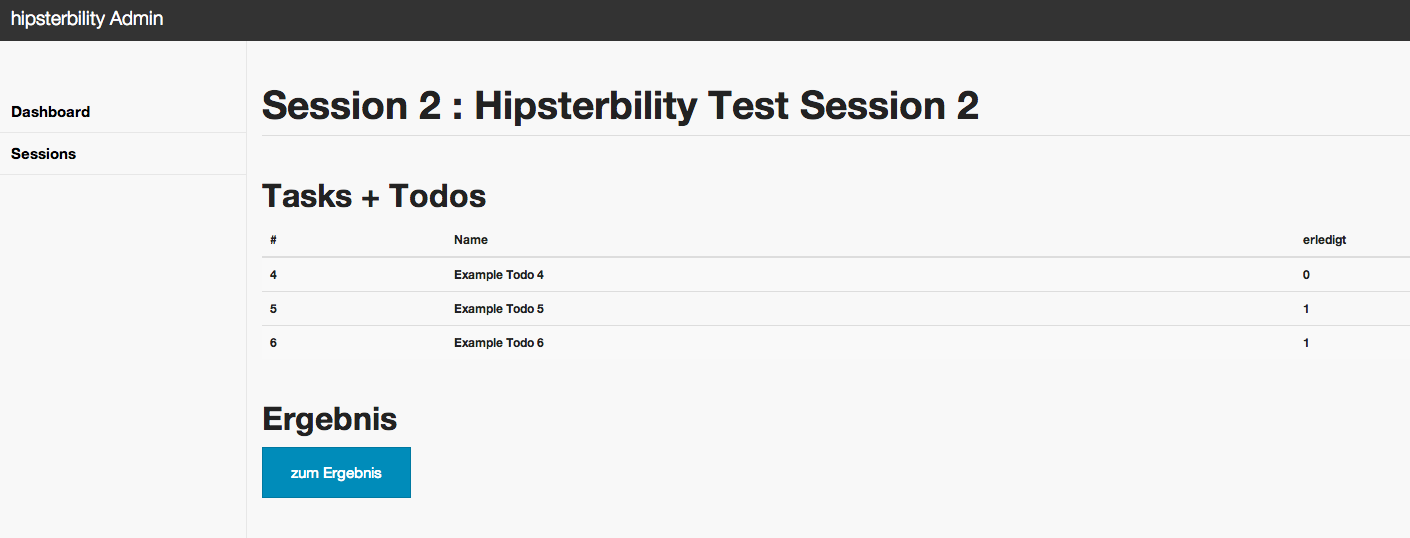
\includegraphics[width=\linewidth,keepaspectratio]{img/session-detail-page.png}
	\caption{Detailansicht einer Testsession}
	\label{fig: session-detail-page}
\end{figure}

\begin{figure}[h!]
	\centering
		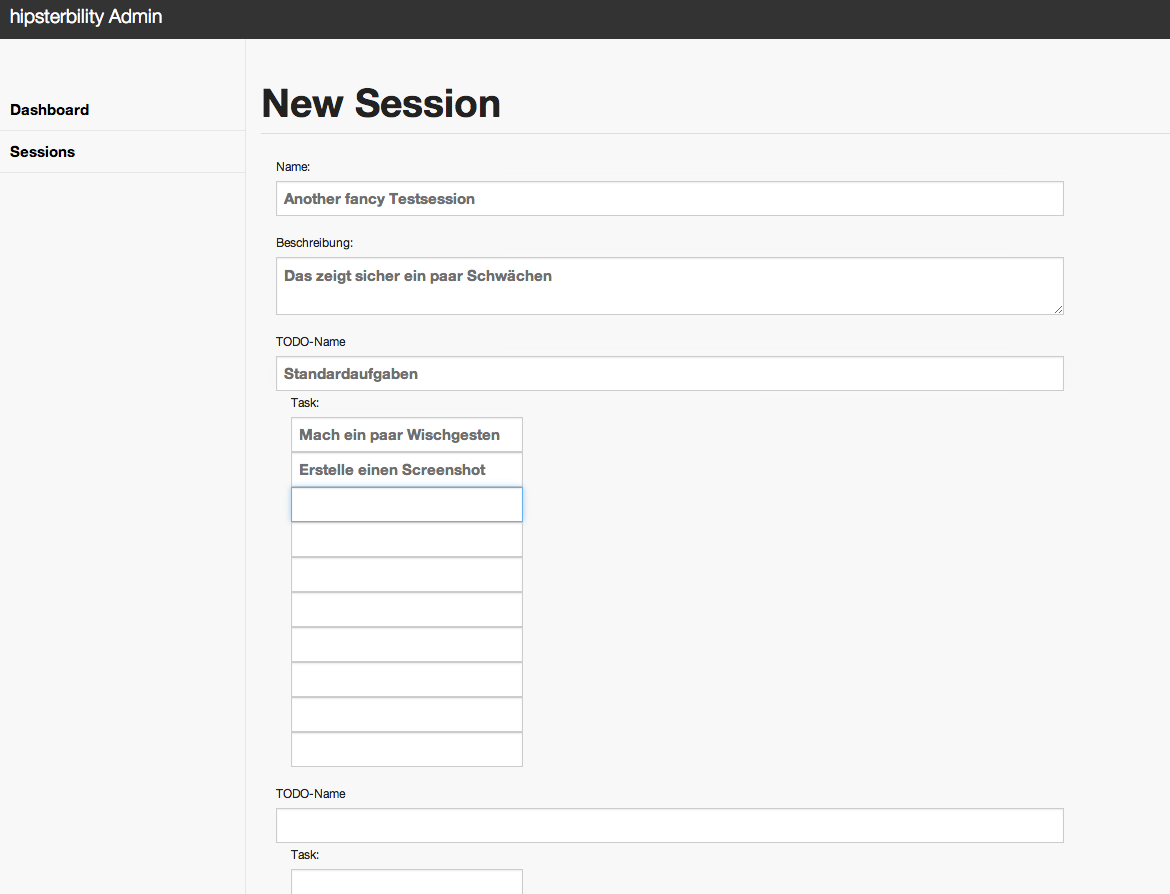
\includegraphics[width=\linewidth,keepaspectratio]{img/session-create-page.png}
	\caption{Neue Session anlegen}
	\label{fig: session-create-page}
\end{figure}

\begin{figure}[h!]
	\centering
		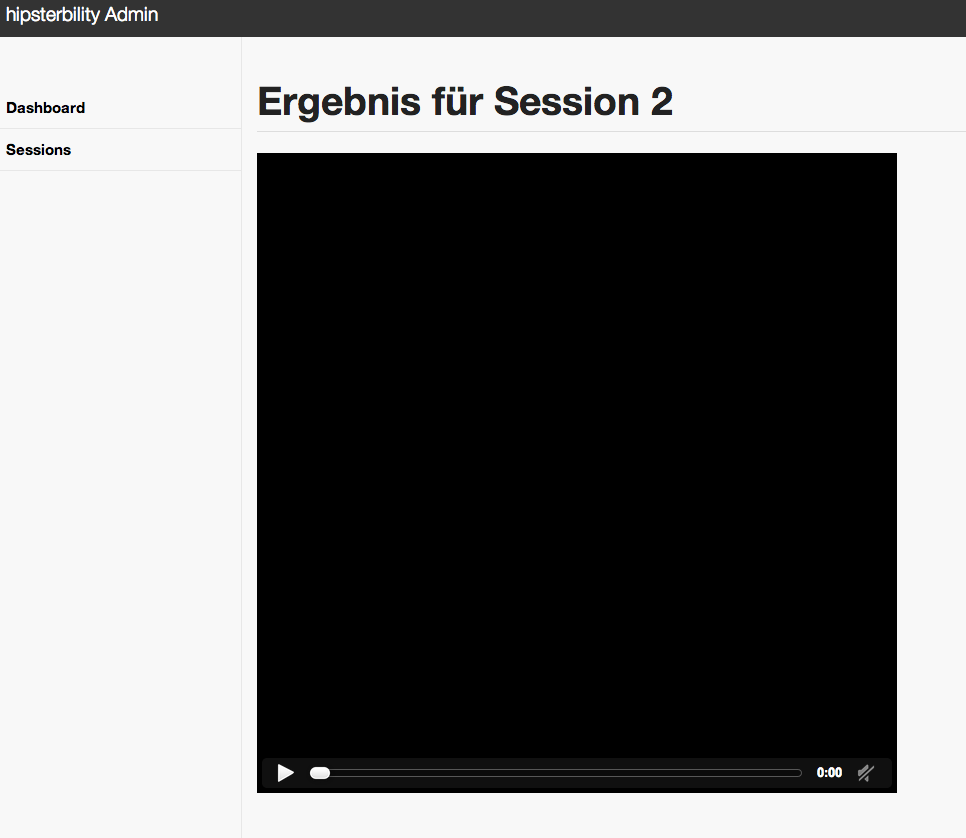
\includegraphics[width=\linewidth,keepaspectratio]{img/session-result-page.png}
	\caption{Web-Ansicht der Ergebnisse}
	\label{fig: session-result-page}
\end{figure}

\subsubsection{API \label{sec: api}}

Neben der webbasierten Verwaltung benötigt der mobile Client eine einfache Anbindung an die Funktionen des Servers. Dafür eignen sich APIs sehr gut. Das Express-Framework bietet sich auch dafür sehr gut an. Nachfolgend werden die API-Routen beschrieben und anschließend wird die Implementierung einer Route beispielhaft gezeigt. 

\subsection{Videoproduktion}

Zur Erstellung der Zwischenergebnisse und des Endergebnisses wird die Open Source-Bibliothek \emph{libav}\footnote{https://libav.org/} verwendet. Genauer wird die darin enthaltene Software \emph{avconv} genutzt um die Bilder und Videos zusammenzufügen. Genauer wird das Kommandozeilenwerkzeug \textit{avconv} benötigt.
% TODO fertig machen.
